\documentclass{article}

% if you need to pass options to natbib, use, e.g.:
\PassOptionsToPackage{square, numbers}{natbib}
% before loading neurips_2020

% ready for submission
% \usepackage{neurips_2020}

% to compile a preprint version, e.g., for submission to arXiv, add add the
% [preprint] option:
%     \usepackage[preprint]{neurips_2020}

% to compile a camera-ready version, add the [final] option, e.g.:
%     \usepackage[final]{neurips_2020}

% to avoid loading the natbib package, add option nonatbib:

\usepackage[preprint]{neurips_2020}
\usepackage{amsmath}
\def\R{\mathbb{R}}
\def\RP{\mathbb{RP}}
\def\Q{\mathbb{Q}}
\def\Z{\mathbb{Z}}
\def\N{\mathbb{N}}
\def\C{\mathbb{C}}
\def\T{\mathcal{T}}
\def\A{\mathbb{A}}
\def\*#1{\mathbf{#1}}

\bibliographystyle{abbrvnat}

\usepackage{xcolor}
\usepackage{graphicx}
\usepackage[utf8]{inputenc} % allow utf-8 input
\usepackage[T1]{fontenc}    % use 8-bit T1 fonts
\usepackage{hyperref}       % hyperlinks
\usepackage{url}            % simple URL typesetting
\usepackage{booktabs}       % professional-quality tables
\usepackage{amsfonts}       % blackboard math symbols
\usepackage{nicefrac}       % compact symbols for 1/2, etc.
\usepackage{microtype}      % microtypography

% \title{Formatting Instructions For NeurIPS 2020}
\title{Meta Reinforcement Learning on Neural Networks}

% The \author macro works with any number of authors. There are two commands
% used to separate the names and addresses of multiple authors: \And and \AND.
%
% Using \And between authors leaves it to LaTeX to determine where to break the
% lines. Using \AND forces a line break at that point. So, if LaTeX puts 3 of 4
% authors names on the first line, and the last on the second line, try using
% \AND instead of \And before the third author name.

\author{%
  Alexander D.~Cai \\
  Harvard College \\
  Cambridge, MA 02138 \\
  \texttt{alexcai@college.harvard.edu} \\
  \And
  Oliver Cheng \\
  Harvard College \\
  Cambridge, MA 02138 \\
  \texttt{ocheng@college.harvard.edu} \\
  % David S.~Hippocampus \\
  % Department of Computer Science\\
  % Cranberry-Lemon University\\
  % Pittsburgh, PA 15213 \\
  % \texttt{hippo@cs.cranberry-lemon.edu} \\
  % examples of more authors
  % \And
  % Coauthor \\
  % Affiliation \\
  % Address \\
  % \texttt{email} \\
  % \AND
  % Coauthor \\
  % Affiliation \\
  % Address \\
  % \texttt{email} \\
  % \And
  % Coauthor \\
  % Affiliation \\
  % Address \\
  % \texttt{email} \\
  % \And
  % Coauthor \\
  % Affiliation \\
  % Address \\
  % \texttt{email} \\
}


\begin{document}

\maketitle

\begin{abstract}
  In the field of reinforcement learning (RL), the subfield of meta-learning has recently gained popularity. Meta-learning proposes to not only learn the policy (which selects actions), but rather a flexible \emph{RL algorithm} which learns the policy. This claims to make the training process more data-efficient and generalizable across tasks. We build off of work from \citet{wang2018pfc} that investigates the implications for biological learning. The structure is as follows: an overarching \emph{policy network} mimics the dopamine system by guiding a fully connected neural network to 
  update its synaptic weights. Over time, the policy network learns an optimal learning rule for which to update
  the weights in the neural network. We empirically find that the optimal policy is to quickly jump to the optimal weights for the training distribution, which does
  not generalize as well as other common learning rules such as Stochastic Gradient Descent (SGD), Weight Perturbation (WP), and Node Perturbation (NP) on teacher-student setups and MNIST.
\end{abstract}

\section{Introduction to Meta-Reinforcement Learning}

In recent years there has been a growing amount of excitement about 
\emph{meta-learning} in order to solve a wider set of problems.
In the typical reinforcement learning setup, an agent interacts with an environment by taking actions and receiving rewards. The goal is to maximize the total reward received. We can 
formalize this as a Markov 
Decision Process (MDP) $\{ \mathcal{S}, \mathcal{A}, P, R, \gamma \}$ where $\mathcal{S}$ is the set of states, $\mathcal{A}$ is the set 
of actions, $P:\mathcal{S} \times \mathcal{A} \to \Delta(\mathcal{S})$ governs the state transitions, and $R: \mathcal{S} \times \mathcal{A} \to \mathbb{R}$ is the reward function. Let 
$\pi_\theta$ be the parameterized policy. 
Thus for some MDP $\mathcal{M}$, the goal is to maximize the mean discounted reward 
\[ \mathcal{J}_{\mathcal{M}}(\theta) = \mathbb{E}_{a_{t=0}^{\infty} \sim \pi_\theta(s_t), s_{t+1}
 \sim P(s_t, a_t)} \left( \sum_t \gamma^t R(s_t, a_{t-1}) \right).\]

This framework gives us a way to view human beings and the nervous system as a 
reinforcement learning program where the human is the agent. One notable trait of the human brain is that it learns and maintains numerous distinct skills, as opposed to typical RL algorithms which can only optimize for a given task. To generalize, we instead seek to develop meta-learning algorithms, 
where rather than optimizing a single policy for a single task,
we aim to learn an RL algorithm which finds optimal policies over a diverse distribution 
of tasks. This idea is motivated by the idea in psychology of 
 ``learning how to learn'' and is conceptually closer to how the brain 
works \cite{wang2018pfc}.

\section{(Multi-Agent) Reinforcement Meta-Learning to find Optimal Learning Rules}


\begin{figure}
  \centering
  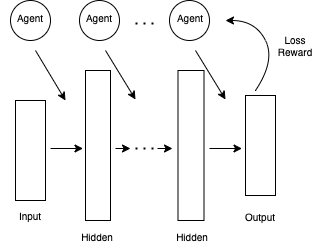
\includegraphics[scale=0.6]{marlnn} 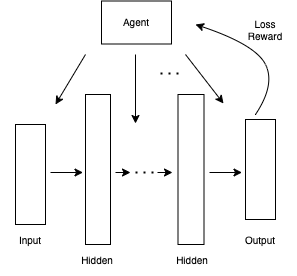
\includegraphics[scale=0.6]{singleagent}
  \caption{Our neural meta-learning paradigm, framed as a multi-agent problem (left) and a single-agent problem (right). We seek to find the parameters $\theta$ which maximize reward, which we define as the negative of the training loss on a fixed training dataset. We do this by optimizing the policy network's parameters using Proximal Policy Optimization \cite{schulman_ppo}. In the multi-agent framing, each agent is in control of a set of weights and can only see the activations of its own weights and those of the previous agent. All agents receive the same total reward. In the single-agent framing, a single agent has complete control and knowledge of all weights.   \label{fig:meta-rl}}
\end{figure}
 

We model neural network training as follows. We aim to optimize the parameters of a ``base'' network $f_{\phi},$ parameterized by $\phi \in \Phi$, to minimize the training error on a dataset. Then, to imitate a model-based dopamine
system which determines which synapses are reinforced, we consider a policy
neural network which will update the weights for the neural net \cite{wang2018pfc, botvinick2019408}. The state space and action space of the MDP thus coincide with $\Phi$.

From here we can construct two different
systems. One is where a single agent gets information on all of the weights,
and can take actions to improve weights accordingly. This is less biologically plausible since it would be difficult
for any neuron in the brain to have access to have all of this data. The second system we consider is setting one agent
for each layer. Each agent has information about the previous layer's weights and activations, and is able to control
the weights to the next layer. In other words, the agent corresponding to the the $\ell$-th layer, $\*x^{(\ell)}$, has control over the weights 
$[\*W^{(\ell)}]_{ij}$. This is more biologically plausible as this would imply each agent need not have connections to all the neurons in 
the network, but rather a local subset of them. Unfortunately, although the second system is conceptually closer to biology, the implementation
with current libraries is shaky at best. Theoretically it would not perform any better than the first system, as each agent has less information
to operate on, and since the policy is a deep neural network, the loss of this information would be a large hindrance to performance.

We use Proximal Policy Optimization (PPO) in order to progressively improve the policy. We can define
our reward as the negative loss for the neural network, thus having smaller absolute loss will be a larger reward, and
PPO will find a policy that optimizes for the largest expected reward. To compute the reward for any given policy, we 
take $T$ different trajectories. For each trajectory $t$ we find how the loss $E_t$ 
decreases after a successive forward passes (1e5 epochs) through the neural 
network with weights specified by the agent/policy network. The reward is 
then transmitted as $\langle - E_t \rangle$ and the policy is updated. This process constitutes a single timestep.

Recall from SGD we have update rules that involve using the gradient to traverse through the loss landscape,
in our case we are learning a learning rule and hence the meta "learning how to learn" concept. The goal is for
the policy to converge to a learning rule that is optimal for the given task, which will not necessarily be SGD
or learning with global error signals that we will look at below, but rather one that is more fine-tuned to the particular
set of problems, for example learning from a teacher with noise or classifying digits in the MNIST dataset.


\paragraph{Code Implementation} The project is implemented using the popular \href{https://www.gymlibrary.dev/}{OpenAI Gym} and \href{https://stable-baselines3.readthedocs.io/en/master/}{Stable Baselines 3} libraries for reinforcement learning \cite{openaigym, sb3}. We implement a custom Gym environment that takes the base neural network architecture as an input, along with the training dataset used for calculating the loss. Then at each timestep, the environment receives a candidate set of weights for the base network, and evaluates its loss on the given dataset.

We attempted to implement a multi-agent environment using the more advanced but flexible \href{https://github.com/thu-ml/tianshou}{Tianshou} library and the \href{https://pettingzoo.farama.org/}{Petting Zoo} library for MARL. This implementation is still a work in progress, but if completed, would allow different agents to control different parts of the base network \cite{tianshou, pettingzoo}.

\section{Comparison to Known Learning Rules}

We compare the policy that is learned from our meta-RL model to accepted learning rules in the literature. SGD converges the quickest, but due to the weight transport problem, is not biologically plausible \cite{mazzoni1991}. More biologically plausible alternatives involve learning from a global error signal, and involve perturbation-type learning rules. Global error signals have been observed in the brain, but it is still under much research exactly how the brain uses these error signals in order to learn and update neurons. We will look at NP and WP. We compare how our new model does for teacher-student learning and learning to classify the MNIST dataset.

\begin{figure}
  \centering
  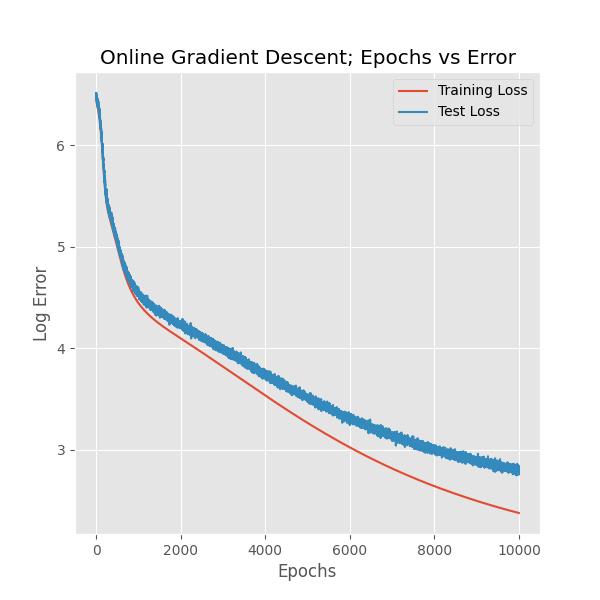
\includegraphics[scale=0.43]{sgd_ts}  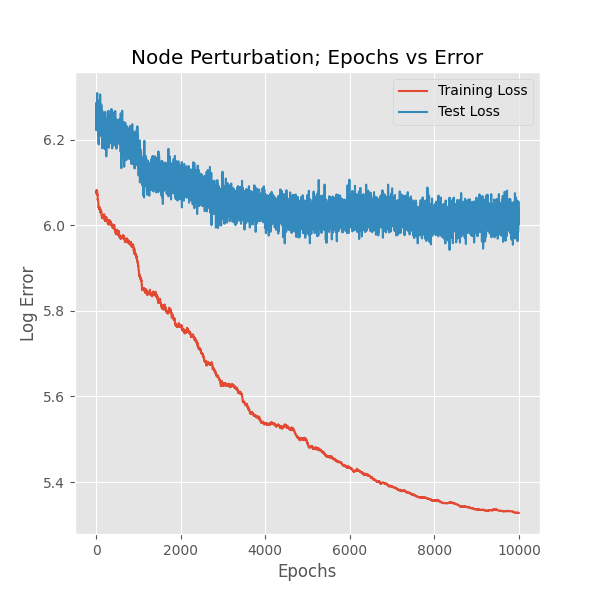
\includegraphics[scale=0.43]{np_ts}  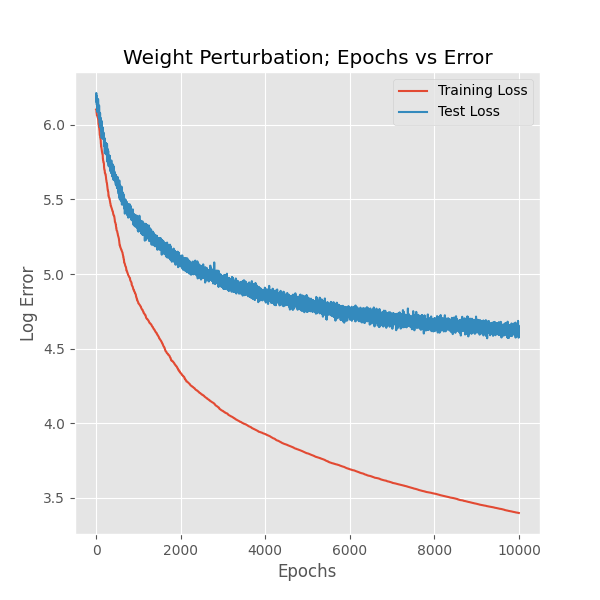
\includegraphics[scale=0.43]{wp_ts}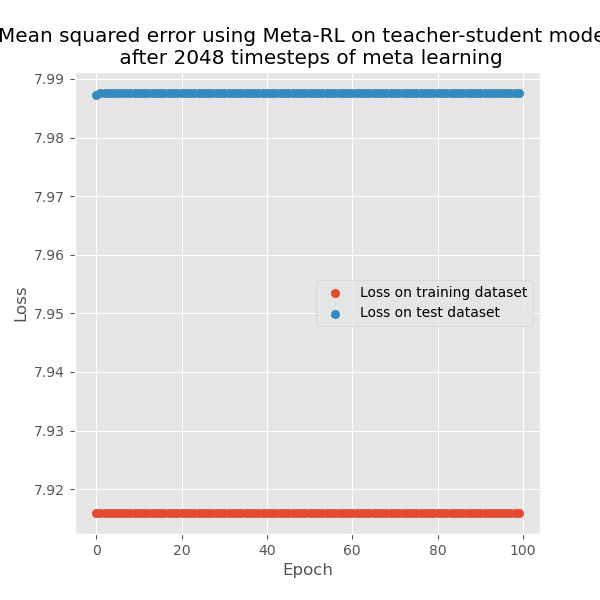
\includegraphics[scale=0.31]{metarl_ts}
  \caption{We find that the policy that the meta-RL system finds is to instantly jump to a certain set of weights, and then perform minimal further updates. The learning rates were chosen to optimize the loss, in the range of $\eta =1.0$ to $0.1$. $\sigma = \frac{1}{L_y L_h}$. \label{fig:teachstudent}}
\end{figure}

The idea behind NP and WP is to take some perturbation $\*\xi$ of either
the weights or the nodes, and then see how that changes the objective or loss \cite{wpnp}. The learning rule update
then corresponds to scaling this perturbation by whether or not it increases or decreases
the loss. Consider a general neural network with $L$ layers and a data set $\{\*x_i^{(0)},\*y_i\}_{i=1}^N$. 
Let $\*W_{\ell} \in \R^{R_{\ell+1} \times R_{\ell}}$ where $R_\ell$ is the number of 
neurons in layer $\ell$. We define the forward pass as
\begin{equation}\label{forward}\*X^{(\ell)} = \sigma\left( \*X^{(\ell-1)}\*W_{\ell-1}^\top\right).\end{equation}
Where $\sigma$ is some non-linearity (we use ReLU). For student teacher, we use the MSE loss 
\begin{equation}
\label{mseloss}
E = \frac{1}{NR_L}\frac 12 \| \*X^{(L)}- \*Y\|^2.
\end{equation}
and for classification into $C = R_L$ classes let 
\begin{equation}
\label{crossentropy}
p(\*x_i^{(L)} = r) = \frac{\exp x_{j,r}^{(L)}}{\sum_{j=1}^C \exp x_{i,j}^{(L)}}.
\end{equation}
We use cross entropy loss for classification
\[E = -\frac 1N \sum_{i=1}^N \sum_{r=1}^C y_r \log p(\*x_i^{(L)} = r) \]
In SGD, we use backpropagation to update the weight parameters by 
\[\Delta_{SGD} \* W_{\ell} = \eta\frac{\partial E}{\partial \*W_{\ell}},\] 
where the chain rule means we 
need to "transport" these values backwards through the neural network. On the other 
hand, in WP/NP, we have two forward passes. For the first, we define the same as \ref{forward}, 
however the second pass for each of WP/NP we introduce a perturbation. For NP, we will let the 
perturbation be a vector $\xi \in \R^{N\times R_{\ell}}$ where all entries are distributed 
i.i.d $\mathcal{N}(0,\sigma)$. We can then define the forward pass as 
\[ \widetilde{\*X}^{(\ell)} = \sigma\left(\widetilde{\*X}^{(\ell-1)}\*W_{\ell -1}^\top + \*\xi^{(\ell)} \right).\]
While for WP we take $\*\Xi^{(\ell)} \in \R^{R_{\ell + 1 }\times R_\ell}$ where all entries are distributed 
i.i.d $\mathcal{N}(0,\sigma)$. 
\[ \hat{\*X}^{(\ell)} = \sigma\left( \hat{\*X}^{(\ell-1)}\left(\*W_{\ell -1} + \*\Xi^{(\ell-1)}\right)^\top  \right).\]
We can then define two errors for each NP and WP respectively. For regression
\[ E_N = \frac{1}{NR_L} \frac 12 \| \widetilde{\* X}^{(L)} - \* Y \|^2 \qquad\qquad E_W = \frac{1}{NR_L} \frac 12 \| \hat{\* X}^{(L)} - \* Y \|^2. \]
For classification
\[E_N  =  -\frac 1N \sum_{i=1}^N \sum_{r=1}^C y_r \log p(\widetilde{\*x}_i^{(L)} = r) \qquad E_W =  -\frac 1N \sum_{i=1}^N \sum_{r=1}^C y_r \log p(\hat{\*x}_i^{(L)} = r).\]
From here we can simply transmit the global error signal $E-E_N$ or $E-E_W$ and update our weights according
to this error signal. In particular, we update parameters as follows for NP
\[ \Delta_{NP} \*W_{\ell} =\frac{\eta}{\sigma} (E-E_N) \sum_{i=1}^{R_{\ell+1}} \*x^{(\ell)}_i \* \xi^{(\ell+1)\top}. \]
While for WP we update as
\[ \Delta_{WP} \*W_{\ell} = \frac{\eta}{\sigma} (E-E_W) \* \Xi^{(\ell)} .\]
 The idea is that perturbations which cause a decrease in the objective will be added to 
 the parameters of the model. In expectation we have that up to a constant
\[ \left\langle \Delta_{NP}\*W_{\ell} \right\rangle_{\*\xi^{(\ell)}}= \left\langle \Delta_{WP}\*W_{\ell} \right\rangle_{\*\Xi^{(\ell)}} =  \Delta_{SGD}\*W_{\ell}.\]
Node and weight perturbation are often used in teacher-student learning cases 
where there is only a single perceptron. Recent work by Hiratani et al. explores node perturbation
in neural networks with a hidden layer, and finds computational and stability issues that
suggest biological implausibility \cite{hiratani2022on}. Nonetheless, these perturbation techniques remain an interesting way
to investigate possible learning rules for neurons. 


\begin{figure}
  \centering
  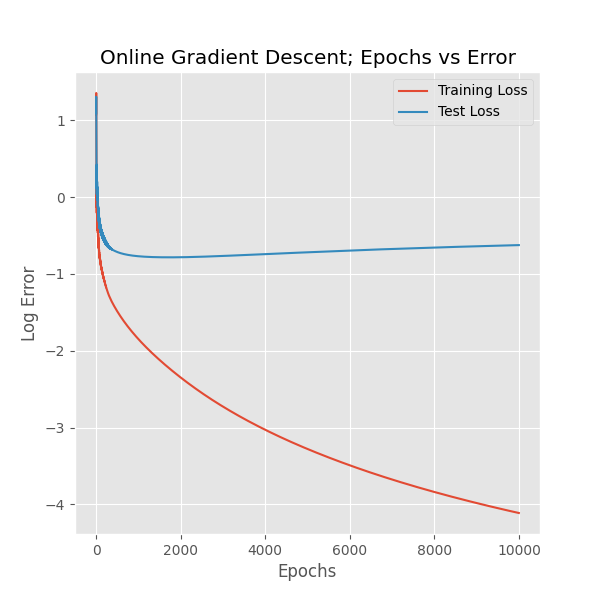
\includegraphics[scale=0.43]{sgd_mnist}  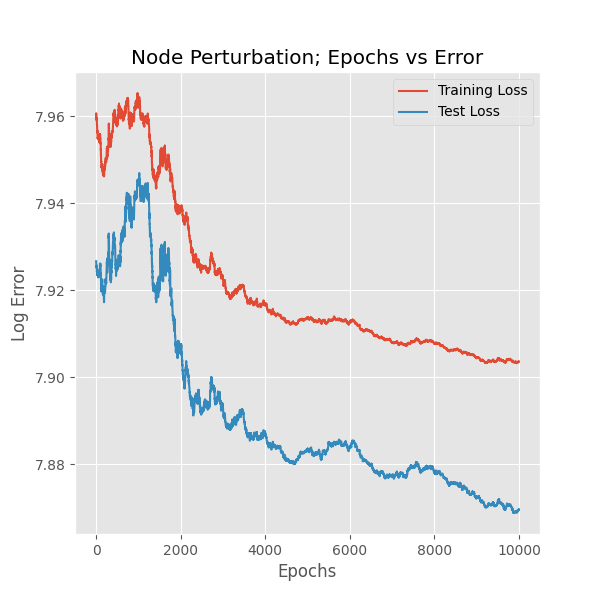
\includegraphics[scale=0.43]{np_mnist}  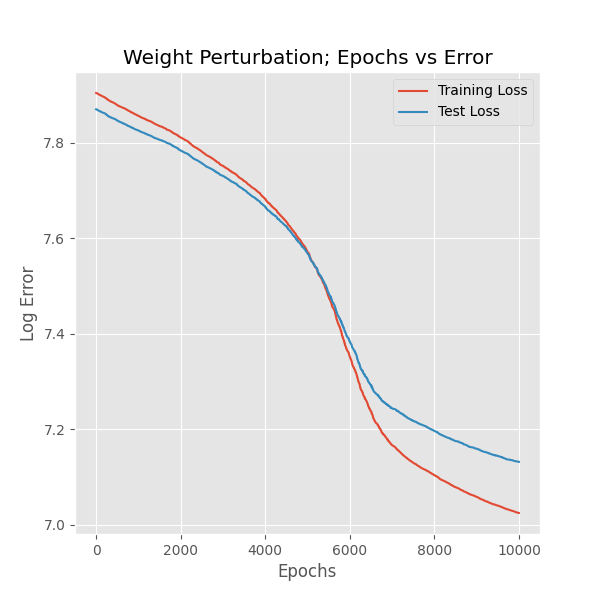
\includegraphics[scale=0.43]{wp_mnist}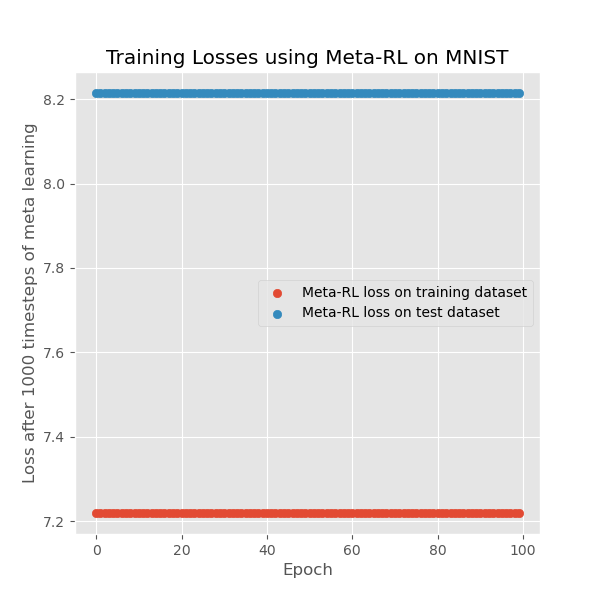
\includegraphics[scale=0.31]{metarl_mnist}
  \caption{Again, we see the Meta-RL NN learn its weights instantly, and as a result have a constant loss for both training and testing. NP is set to $\eta = 10^{-4}$, which is unstable. NP will converge for $\eta\ll 10^{-6}$, but the number of epochs needed to make any reasonable progress was too high to be computationally feasible. $\sigma = \frac{1}{L_y L_h}$.\label{fig:mnist}}
\end{figure}



\paragraph{Training on Student-Teacher (Fig. \ref{fig:teachstudent})} For the student-teacher model, we consider a neural network with one hidden layer. We set the three layer's widths as $L_x = 10, L_h = 100, L_y = 10$. We have a teacher with a hidden set of weights $\*W^*_h, \*W^*_y$ that generates a dataset $N=512$ with noise $\*\zeta_i \in \R^{L_y}$ for $i=1,\ldots, N$, where each element of $\*\zeta_i$ is i.i.d $\mathcal{N}(0, \sigma_t)$. For our cases we set $\sigma_t = 0.01$, as node-perturbation is noisy and unstable otherwise. We define our dataset as $\{\*x_i^{(0)},\*y_i\}_{i=1}^N$ where each element of $\*x_i$ is i.i.d standard normal, and 
\[ \*y_i = \sigma\left(\sigma(\*x_i \*W^{*\top}_h)\*W_y^{*\top}\right) + \*\zeta_i. \]
We use ReLU as the non-linearity for $\sigma$. We are thus optimizing a single-hidden layer neural network 
\[ \hat{\*y}_i =  \sigma\left(\sigma(\*x_i \*W^{\top}_h)\*W_y^{\top}\right).\]
We use MSE loss as in \ref{mseloss}.


\paragraph{Training on MNIST (Fig. \ref{fig:mnist})} Going to MNIST, the problem becomes much more noisy. 
In order to decrease noise, we first preprocess by standardizing and projecting the
data onto the first 10 principal components ($\sim99\%$ of the variance), and decrease the learning rate 
by a factor of 100. It is also necessary to increase the hidden layer width $L_h = 1000$, as otherwise the model did not
have sufficient complexity. We train on a subset of the data $N=512$. We use the same single-hidden layer architecture, with cross entropy loss as in \ref{crossentropy} with $C=10$ for the 10 different digits. As observed by Hiratani et al., the amount of training time required 
for these global error signal models to converge for MNIST is much higher ($10^5$) which was unfeasible due to computational reasons \cite{hiratani2022on}.
We find the accuracy to be decent (50\%) but clearly not optimized as SGD by itself can reach $80\%$ testing accuracy on 10
principal components Fig. \ref{fig:mnistacc}. In order to run without weights exploding, we standardized the weights at each step, thereby providing more stability at the cost of expressivity. 

\begin{figure}
  \centering
  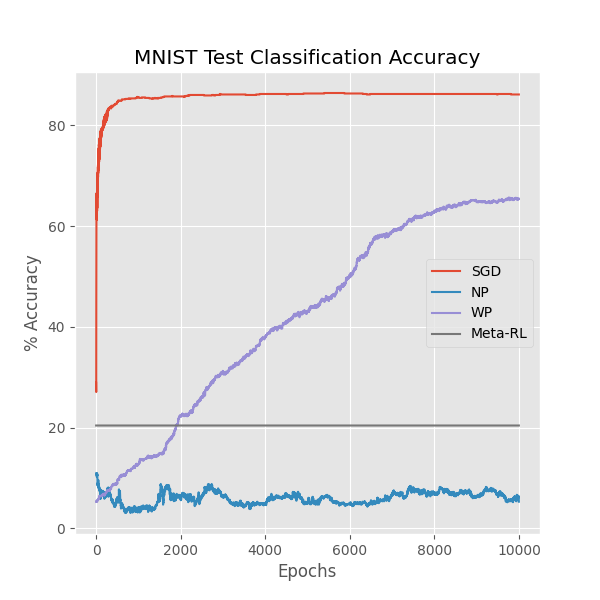
\includegraphics[scale=0.6]{acc}  \caption{Test accuracy for Meta-RL is constant due to the policy network choosing the optimal weights during training instantly. NP is under performing due to being excessively noisy.  \label{fig:mnistacc}}
\end{figure}


We found that one of the issues in our experiment was the tendency for the policy to choose a 
learning rule that updated the weights according to exactly the optimal weights of a training example, 
and hence resulted in substantial overfitting. This could be balanced
by choosing more trajectories for each timestep and training for a longer period. 
\section{Conclusion and Further Steps}

\paragraph{Meta-Reinforcement Learning in the Brain} Wang et al. discussed the 
a notion of "meta-learning" in the brain where the prefrontal cortex acts as a recurrent neural network which triggers actions
and internally holding a notion of the value of a state. Phasic Dopamine (DA) is suggested to act in a similar way to
how our policy network changed the weights of the neural network. In particular, the synaptic weights are adjusted
by the model-free RL DA system, where DA releases are similar to the reward prediction error in temporal-difference 
RL algorithms. The reason why meta-RL fits this structure better than standard RL is because of the ability to use past 
experiences the brain has in order to learn an optimal policy, and this is clearly seen in human and animal brains \cite{wang2018pfc}.

\paragraph{Computation Limits and Further Steps} Wang et al. were able to achieve results relating meta-RL to the prefrontal cortex and 
dopamine system with the large computational power of DeepMind \cite{wang2018pfc}. 
Our results show how the parameter size of models of this nature must be substantially 
larger in order to achieve results that are generalizable to even classic tasks such as
MNIST or student-teacher. Further steps in this research include exploring a wider distribution
of tasks $p(\mathcal{T})$ in order to harness the generalizability of meta-RL. Given more computational
power it would also be interesting to see if the multi-agent meta-RL system has promise to generalize
more as the optimal weights would be less clear due to the lack of information.

Code for this project can be found at \url{https://github.com/RubberNoodles/meta-MARL-neuronal-NN}.

\bibliography{sample} 
\end{document}
